
\subsection{{Description}}

	{The seven-segment display in this logic circuit serves to visually represent the hexadecimal outputs of the ALU operation based on initial inputs.}
	
	{Additionally, depending on the control unit, separate seven-segment units display integer representations of student ID values.}
	
	{This display mechanism provides a tangible and readable output, aiding in the interpretation of both ALU results and student identification information in the digital system.}

\subsection{{Truth Table}}

	\begin{table}[H]
		\centering
		\begin{tabular}{|c|c|c|c|c|}
		\hline
		\hline
			\textit{A} & \textit{B} & \textit{C} & \textit{D} & \textit{Visual Output} \\ 
			\hline
			\hline
			0 & 0 & 0 & 0 & 0 \\ 
			\hline
			0 & 0 & 0 & 1 & 1 \\ 
			\hline
			0 & 0 & 1 & 0 & 2 \\ 
			\hline
			0 & 0 & 1 & 1 & 3 \\ 
			\hline
			0 & 1 & 0 & 0 & 4 \\ 
			\hline
			0 & 1 & 0 & 1 & 5 \\ 
			\hline
			0 & 1 & 1 & 0 & 6 \\ 
			\hline
			0 & 1 & 1 & 1 & 7 \\ 
			\hline
			1 & 0 & 0 & 0 & 8 \\ 
			\hline
			1 & 0 & 0 & 1 & 9 \\ 
			\hline
			1 & 0 & 1 & 0 & A \\ 
			\hline
			1 & 0 & 1 & 1 & b \\ 
			\hline
			1 & 1 & 0 & 0 & C \\ 
			\hline
			1 & 1 & 0 & 1 & d \\ 
			\hline
			1 & 1 & 1 & 0 & E \\ 
			\hline
			1 & 1 & 1 & 1 & F \\ 
		\hline
		\hline
		\end{tabular}
		\caption{Truth Table for the Seven Segment Display Unit}
	\end{table}

\subsection{{Block Diagram}}

	\begin{figure}[H]
    		\centering
    		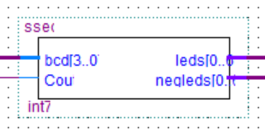
\includegraphics[width=10cm]{Pictures/SSEG.png}
    		\caption{{Block Diagram for the Seven Segment Display Unit}}
    		\label{}
	\end{figure}

%\subsection{{Timing Diagram}}

	{}

